%!TeX program = pdflatex
\documentclass{scrbook}


\usepackage{setspace}
\KOMAoptions{ twoside=true, open=any, headings=optiontoheadandtoc,parskip=true,fontsize=12pt,parskip=half-}
\usepackage{geometry}
\geometry{
	paperwidth=210mm,
	paperheight=297mm,
	layout=a4paper,
	lmargin=23mm, % margin auf der rechten Seite
	rmargin=25mm, % margin auf der linken Seite
	tmargin=18mm,
	textheight=250mm,
	textwidth=154mm,
	includefoot,
	footskip=30pt,
	layoutoffset=3mm
}




%%%%%% Print %%%%%%%%%%%%%%%%%%%%%%%%%%%%%%%%%%%%%%%%%%%%%%%%%%%%%%%%

% Lege die ICC-Datei PSOcoated_v3.icc ins Projektverzeichnis
%\usepackage[x-4]{pdfx} % erzeugt PDF/X-4 mit OutputIntent
% pdfx nimmt standardmäßig die im Projekt liegende ICC als OutputIntent, z. B. PSOcoated_v3.icc

%%%%%% Portraits %%%%%%%%%%%%%%%%%%%%%%%%%%%%%%%%%%%%%%%%%%%%%%%%%%%%

\usepackage{float}
\usepackage{wrapstuff}
\usepackage{wrapfig}


%%%%%% Section titles %%%%%%%%%%%%%%%%%%%%%%%%%%%%%%%%%%%%%%%%%%%%%%%

\setcounter{secnumdepth}{0}
\setcounter{tocdepth}{4}

\RedeclareSectionCommand[
	afterskip = {0.4ex plus 0.2ex},
	beforeskip = {-1ex plus -1ex minus -.2ex},
	font={\LARGE},
]{section}

\RedeclareSectionCommand[
	afterskip = {.4ex plus .2ex},
	beforeskip = {-0.25ex plus -1ex minus -.2ex},
	font={\Large},
]{subsection}
	
\DeclareNewSectionCommand[
	afterskip = {.4ex plus .2ex},
	beforeskip = {-0.25ex plus -1ex minus -.2ex},
	indent=0pt,
	font={\LARGE},
	style=section,
	level=1,
	tocindent=0pt,
	toclevel=1,
	tocnumwidth=2em,
	tocstyle=chapter,
]{sectionPart}

\RedeclareSectionCommand[
afterskip = {-1em},
beforeskip = {0ex plus -1ex minus .2ex},
runin=false,
]{paragraph}

\setparsizes{0pt}%infdent
{9pt}%vskip
{0pt plus 1fil}


%%%%%% Section headings %%%%%%%%%%%%%%%%%%%%%%%%%%%%%%%%%%%%%%%%%%%%

\usepackage{ifthen}
\newcounter{secautolabel}
\AddtoDoHook{heading/endgroup}{\setautolabel}
\newcommand*{\setautolabel}[1]{%
  	\stepcounter{secautolabel}%
  	\label{sec:autolabel:\thesecautolabel}%
	\def\sname{#1}
	\ifthenelse{\equal{#1}{sectionPart}}{
		\def\sname{section}
	}{}
  	\expandafter\xdef\csname \sname title\endcsname{%
    	\noexpand\nameref{sec:autolabel:\thesecautolabel}%
  	}%
}


%%%%%% Font, Encoding etc. %%%%%%%%%%%%%%%%%%%%%%%%%%%%%%%%%%%%%%%%%%

\usepackage[utf8]{inputenc}
\usepackage[T1]{fontenc}
\usepackage[ngerman]{babel}
\usepackage{amsmath,amsfonts,amssymb}
\usepackage[default,light,lf]{FiraSans}
\usepackage{pifont}


%%%%%% Schritsatz %%%%%%%%%%%%%%%%%%%%%%%%%%%%%%%%%%%%%%%%%%%%%%%%%%%%

% Blocksatz aktiv + bessere Trennung
\usepackage{microtype}        % Mikrotypografie für schönere Zeilen
\emergencystretch=2em         % Puffer gegen overfull lines

% Flattersatz & Trennung aus
%\usepackage{ragged2e}
%\AtBeginDocument{\RaggedRight}      % global linksbündig (kein Blocksatz)
%\usepackage[none]{hyphenat}         % Silbentrennung aus
%\emergencystretch=1em               % etwas Puffer gegen overfull lines
%\setlength{\RaggedRightParindent}{0pt}


%%%%%% Colors %%%%%%%%%%%%%%%%%%%%%%%%%%%%%%%%%%%%%%%%%%%%%%%%%%%%%%%

\usepackage{xcolor,colortbl}

\definecolor{fscolor}{RGB}{11,161,226}
\definecolor{petrol}{HTML}{216477}
\definecolor{lecegreen}{HTML}{0aa3e4}


%%%%%% tikz %%%%%%%%%%%%%%%%%%%%%%%%%%%%%%%%%%%%%%%%%%%%%%%%%%%%%%%%%

\usepackage{tikz}
\usetikzlibrary{calc}
\usetikzlibrary{shapes.geometric}
\usetikzlibrary{decorations}


%%%%%% Tabellen %%%%%%%%%%%%%%%%%%%%%%%%%%%%%%%%%%%%%%%%%%%%%%%%%%%%%

\usepackage{tabularx}
\usepackage{makecell}
\usepackage{tabularray}
\usepackage{multicol}
%\usepackage{tocbasic}        % Inhaltsverzeichnis verändern schiebt es nach unten oder oben

%%%%%% Sonstiges %%%%%%%%%%%%%%%%%%%%%%%%%%%%%%%%%%%%%%%%%%%%%%%%%%%%

\usepackage{qrcode}

\usepackage[]{graphicx}

\usepackage[export]{adjustbox}% http://ctan.org/pkg/adjustbox

\usepackage{caption}
\usepackage{subcaption}

\usepackage{array}
\usepackage{forarray}
\usepackage{forloop}

\usepackage{enumitem}
\usepackage{etoolbox}
\usepackage[german=quotes]{csquotes}
\usepackage{scrlayer-fancyhdr}

\usepackage{microtype}
\usepackage{lipsum}           % Platzhaltertext
\usepackage{pdfpages}         % Für PDF-Einbindung
\usepackage{setspace}



% URLs besser umbrechen (Option muss vor hyperref rein)
\PassOptionsToPackage{hyphens}{url}


\usepackage[
	linktoc=black,
	linkcolor=.,
	urlcolor=fscolor,
	breaklinks=true,
	colorlinks,
	bookmarks,
	plainpages=false,
	citecolor=gray,
]{hyperref}
\urlstyle{same}
\usepackage{cleveref}

% URL-Umbrüche noch flexibler
\Urlmuskip=0mu plus 2mu


% Checkliste
\newlist{todolist}{itemize}{2}
\setlist[todolist]{label=$\square$}


\newcounter{pagehead}


%%%%%%%%%%%%%%%%%% Citations %%%%%%%%%%%%%%%%%%%%%%%%%%%%%%%%%%%%%%%%
\usepackage[backend=biber,style=authoryear,maxcitenames=2,maxbibnames=99]{biblatex}
\addbibresource{literatur.bib}

\fancyhead[OR,EL]{}
\fancyhead[ER]{\tikzheade}
\fancyhead[OL]{\tikzhead}
\renewcommand{\headrulewidth}{0pt}
\renewcommand{\footrulewidth}{0pt}

\pagestyle{fancy}
\fancypagestyle{plain}{
	\renewcommand{\headrulewidth}{0pt}
	\fancyhf
	%	\fancyfoot[C]{}
}
\usetikzlibrary{calc}

\newcommand*\tikzhead{%
	\begin{tikzpicture}[remember picture,overlay]
		\node[%
			fill = fscolor,%
			xshift=-0.35cm,yshift=-0.3cm,
			anchor=east,%
			font = \color{white},%
			text width = 13mm,%
			inner sep = 3pt,%
			%inner xsep=1em,
			align= left,
			minimum height=15pt,
		] at ($(current page.north east)+(6pt,-1)$) {\phantom{a}\arabic{page}};
		
		\node[%
			anchor=east,%
			xshift=-0.5cm,yshift=-0.3cm,
			inner sep = 3pt,
			font=\color{fscolor},%
		] at ($(current page.north east)+(-1.25,-1)$) {\sectiontitle};
	\end{tikzpicture}
}

\newcommand*\tikzheade{%
	\begin{tikzpicture}[remember picture,overlay]
		\node[%
			xshift=0.35cm,yshift=-0.3cm,
			fill = fscolor,%
			anchor=west,%
			font = \color{white},%
			text width = 13mm,%
			inner sep = 3pt,
			%inner xsep=1em,
			align= right,
			minimum height=15pt,
		] at ($(current page.north west)-(6pt,1)$) {\arabic{page}\phantom{a}};
		
		\node[%
			anchor=west,%
			xshift=0.5cm,yshift=-0.3cm,
			inner sep = 3pt,
			font=\color{fscolor},%
		] at ($(current page.north west)+(1.25,-1)$) {\sectiontitle};
	\end{tikzpicture}
}


\newcommand{\partarrow}{%
	\begin{tikzpicture}[scale=0.3]
		\draw[line width = 3pt] (0,0) -- (2,-1) -- (0,-2);
	\end{tikzpicture}
	
}

\newcommand{\PART}[1]{
	\newpage
	\thispagestyle{empty}
	\addcontentsline{toc}{chapter}{#1}
	{\pagecolor{fscolor}
		\begin{tikzpicture}[remember picture, overlay]
			\node[%
			anchor=north west, 
			font=\fontsize{36}{2em}\selectfont\color{white}%
			] at (0.5, -4)
			{%
				\begin{tikzpicture}
					\node[anchor=north east] at (0,-0.16) {\partarrow};
					\node[%
						anchor=north west,%
						align=flush left,%
						text width = 9 cm,%
						execute at begin node=\setlength{\baselineskip}{2ex}%
					] at (-0.6,0) {\bfseries #1};
				\end{tikzpicture}
			};
	\end{tikzpicture}}
	
	\newpage
	\pagecolor{white}
}

\newcommand{\Paragraph}[1]{\paragraph*{#1}}
\newcommand{\vorlesungsdaten}[5]{%
	\begin{tabbing}%
		\hspace*{2.5cm}\= \kill%
		\ifstrempty{#1}{}{Vorlesung: \> #1 \\}%
		\ifstrempty{#2}{}{Zeit: \> #2 \\}%
		\ifstrempty{#3}{}{Ort: \> #3 \\}%
		\ifstrempty{#4}{}{Übungen: \> #4 \\}%
		\ifstrempty{#5}{}{Sprechstunde: \> #5}%
	\end{tabbing}
}

\newcommand{\Par}[1]{%
	\textbf{#1}

	\vspace{-1em}%
}




%%%%%%% Links %%%%%%%%%%%%%%%%%%%%%%%%%%%%%%%%%%%%%%%%%%%%%%%%%%%%%%

\NewDocumentCommand{\link}{O{#2}m}{%
	\vspace{-4pt}%
	\begin{center}%
		\href{#2}{#1}%
	\end{center}%
	\vspace{-4pt}%
}
\NewDocumentCommand{\inlinelink}{O{#2}m}{\href{#2}{#1}}


%%%%%%% Bilder %%%%%%%%%%%%%%%%%%%%%%%%%%%%%%%%%%%%%%%%%%%%%%%%%%%%%

\newcommand{\portrait}[3][0.3]{%
	\begin{wrapstuff}[r,belowsep=-2cm+#3]
		\includegraphics[width=#1\textwidth,keepaspectratio]{./content/photos/#2}
	\end{wrapstuff}
}

\newcommand{\comic}[2][5cm]{%
	\begin{center}
		\includegraphics[height=#1,keepaspectratio]{./content/comics/#2}
	\end{center}
}


%%%%%%% Tabellen %%%%%%%%%%%%%%%%%%%%%%%%%%%%%%%%%%%%%%%%%%%%%%%%%%%%

\newcommand{\coursecell}[3]{\makecell{{\bfseries #1} \\ (#2\ CP, #3\ \%)}}
\newcommand{\coursecellTwolines}[4]{\makecell{{\bfseries #1} \\ {\bfseries #2} \\ (#3\ CP, #4\ \%)}}
\newcommand{\coursecellTwolinesLP}[4]{\makecell{{\bfseries #1} \\ {\bfseries #2} \\ (#3\ LP, #4\ \%)}}
\newcommand{\coursecellThreelines}[5]{\makecell{{\bfseries #1} \\ {\bfseries #2} \\ {\bfseries #3} \\ (#4\ CP, #5\ \%)}}
\newcommand{\coursecellThreelinesLP}[5]{\makecell{{\bfseries #1} \\ {\bfseries #2} \\ {\bfseries #3} \\ (#4\ LP, #5\ \%)}}

\newcommand{\coursecellmt}[4]{\makecell[c]{{\bfseries #1  (#2\ LP, #3\ \%)} \\ #4}}

\newcommand{\celltopbot}[2]{\makecell{{\bfseries #1 \\ #2\ LP}}}

\newcommand{\tabitem}{~~\llap{\textbullet}~~}

\newcommand{\rotateTH}[2][1.6cm]{\rotatebox[origin=c]{90}{\parbox{#1}{\begin{center}\bfseries #2\end{center}}}}


%%%%%%% Checkliste %%%%%%%%%%%%%%%%%%%%%%%%%%%%%%%%%%%%%%%%%%%%%%%%%%

\newcommand{\cmark}{\ding{51}}%
\newcommand{\xmark}{\ding{55}}%
\newcommand{\done}{
	\makebox[0pt][l]{$\square$}\raisebox{.15ex}{\hspace{0.1em}\Large$\checkmark$}\hspace{-0.4em}%
}

%%%%%% Sonstiges %%%%%%%%%%%%%%%%%%%%%%%%%%%%%%%%%%%%%%%%%%%%%%%%%%%%%


\newcommand{\druckrand}{\draw[ultra thin, dotted, dash pattern=on 4pt off 4pt] ($(current page.north west)+(3mm,-3mm)$) rectangle ($(current page.south east)+(-3mm,3mm)$);}
%\renewcommand{\druckrand}{\node at (0,0) {};}

\onehalfspacing
\raggedbottom

\begin{document}


\begin{titlepage}
    \centering
    \vspace*{2cm}

    {\LARGE\textbf{Warum ist Gras grün?}\par}
    \vspace{2cm}

    {\large Bachelorarbeit zur Erlangung des akademischen Grades\\
    Bachelor of Science (B.Sc.)\par}
    \vspace{2cm}

    \begin{flushleft}
        \textbf{Prüfling:} Max Musterjung\\
        \textbf{Matrikelnummer:} 1234567\\
        \textbf{Studiengang:} Angewandte Naturwissenschaften\\
        \textbf{Hochschule:} Universität Musterstadt
    \end{flushleft}

    \vfill

    \begin{center}
        \textbf{Erstprüfer:} Prof. Dr. Max Mustermann\\
        \textbf{Zweitprüferin:} Prof. Dr. Gisela Musterfrau
    \end{center}

    \vspace{1cm}
    {\large \today\par}
\end{titlepage}


% Inhaltsverzeichnis
\clearpage
\begingroup
  \renewcommand{\sectiontitle}{Inhaltsverzeichnis}%
  % \pagestyle{scrheadings}% nur falls du vorher umgestellt hattest
  \tableofcontents
\endgroup

\chapter{Einleitung}

\section{Motivation und Kontext}
Gras ist ein allgegenwärtiger Bestandteil unserer natürlichen Umgebung. Es bedeckt große Flächen in Gärten, Parks, Wiesen und landwirtschaftlich genutzten Flächen und erfüllt dabei vielfältige ökologische und ästhetische Funktionen. Trotz dieser Allgegenwärtigkeit stellen sich viele Menschen kaum die Frage, warum Gras eigentlich seine charakteristische grüne Farbe hat, eine Eigenschaft, die wir oft als selbstverständlich wahrnehmen.

\section{Physikalisch-biochemischer Rahmen}
Die Farbe einer Pflanze ist keineswegs ein bloßes Zufallsprodukt, sondern Ergebnis komplexer physikalischer und biochemischer Prozesse. Insbesondere das Zusammenspiel zwischen Licht, Pflanzenzellen und spezifischen Farbstoffen wie Chlorophyll führt zu dem visuellen Eindruck, den wir als „grün“ wahrnehmen. Die Ursache liegt unter anderem in der Art und Weise, wie elektromagnetische Wellen von bestimmten Molekülen absorbiert, reflektiert oder durchgelassen werden.

\section{Zielsetzung der Arbeit}
Ziel dieser Arbeit ist es, die grundlegenden Mechanismen zu beleuchten, die dazu führen, dass Gras grün erscheint. Dazu werden sowohl die physikalischen Eigenschaften des Lichts als auch die biochemischen Prozesse in der Pflanze untersucht. Im Zentrum steht die Rolle des Farbstoffs Chlorophyll, der für die Absorption bestimmter Wellenlängen des Lichts verantwortlich ist und damit die entscheidende Basis für die Photosynthese bildet. Darüber hinaus wird auf die evolutionäre Bedeutung der Farbgebung eingegangen, um zu zeigen, dass selbst eine scheinbar einfache Eigenschaft wie „Grünsein“ eine Vielzahl biologischer Funktionen erfüllen kann.

% Optional: prägnante Leitfragen als Orientierung
\subsection{Leitfragen}
\begin{itemize}
  \item Welche optischen und physiologischen Mechanismen führen zur grünen Erscheinung von Gras?
  \item Welche Rolle spielen Chlorophyll und akzessorische Pigmente im Absorptionsspektrum?
  \item Wie lässt sich die Farbwirkung im Kontext von Ökologie und Evolution einordnen?
\end{itemize}

\section{Aufbau der Arbeit}
Die Arbeit gliedert sich in mehrere Abschnitte. Zunächst wird ein theoretischer Hintergrund zu Licht, Farbwahrnehmung und pflanzlicher Pigmentierung geschaffen. Anschließend folgt eine detaillierte Betrachtung der Photosynthese und ihrer physikalischen Rahmenbedingungen. Im Anschluss werden mögliche Deutungen und Erweiterungen diskutiert, bevor die Ergebnisse im abschließenden Kapitel zusammengefasst werden.

\chapter{Methodik und Stand der Forschung}

\section{Ziel und Studiendesign}
Ziel dieses Kapitels ist es, die Vorgehensweise der Literaturauswertung transparent zu machen und den aktuellen Stand der Forschung strukturiert zu synthetisieren. Der Fokus liegt auf Mechanismen der Farbentstehung bei Gräsern, insbesondere Pigmentabsorption, Blattoptik, Photoprotektion und Wahrnehmungsaspekte. Die Arbeit folgt einer narrativen, qualitativ-analytischen Synthese auf Basis gezielter Literaturrecherche.

\section{Literaturrecherche}
Die Recherche erfolgte iterativ in einschlägigen Datenbanken und Suchmaschinen. Die Kombination aus kontrollierten Begriffen und freien Suchphrasen zielte auf Übersichtsarbeiten und zentrale Primärstudien.

\subsection{Datenbanken und Suchhorizont}
\begin{tblr}{
  colspec={lX},
  row{1} = {font=\bfseries},
  rows = {abovesep=2pt, belowsep=2pt}
}
Quelle / Datenbank & Rahmen \\
Google Scholar      & Breite Abdeckung, Vorselektion über Titel/Abstract. \\
Web of Science      & Fachlich kuratierte Journals, Zitationsnetzwerke. \\
Institutionelle Repositorien & Zugriff auf historische Primärquellen und Lehrmaterial. \\
\end{tblr}

\subsection{Suchstrings (Beispiele)}
\begin{itemize}
  \item \textit{“chlorophyll absorption”} \textit{AND} \textit{“green gap”} \textit{AND} \textit{“leaf optics”}
  \item \textit{“photosystem electron transport”} \textit{AND} \textit{“ATP NADPH”}
  \item \textit{“green light canopy penetration”} \textit{AND} \textit{“shade tolerance”}
  \item \textit{“carotenoids photoprotection”} \textit{AND} \textit{“nonphotochemical quenching”}
\end{itemize}

\subsection{Ein- und Ausschlusskriterien}
\begin{tblr}{
  colspec={lX},
  row{1} = {font=\bfseries},
  rows = {abovesep=2pt, belowsep=2pt}
}
Einschluss & Peer-reviewte Artikel, Kapitel oder Standardlehrwerke mit direktem Bezug zu Pigmentabsorption, Blattoptik, Photosynthesekinetik oder Wahrnehmungsaspekten. \\
Ausschluss & Rein technische Anwendungsberichte ohne Bezug zu Mechanismen; Studien ohne nachvollziehbare Methodik; Duplikate. \\
\end{tblr}

\subsection{Screening und Auswahl}
Zunächst wurden Titel und Abstract gescreent (Relevanz, Qualität). Danach Volltexte geprüft und bibliographische Rückwärtssuche genutzt. Zentralbelege wurden priorisiert, ergänzend wurden Übersichtsarbeiten herangezogen \parencite{meyer2018photosynthese, schmidt2015chlorophyll, gao2010lightabsorption, zhao2012chlorophyll, renoult2017evolution}.

\section{Datenextraktion und Auswertung}
Für jedes Werk wurden Kernaussagen zu (i) Pigmenten und Spektren, (ii) Blattoptik/Gewebe, (iii) Photoprotektion und (iv) Wahrnehmung erfasst. Widersprüche wurden tabellarisch festgehalten und in der Diskussion adressiert. Die Synthese folgt einem mechanistischen Raster (vom Photon zum visuellen Eindruck) und verknüpft Befunde über Skalen (Blatt, Bestand, Wahrnehmung).

\section{Bias und Limitationen}
Die narrative Synthese ist anfällig für Auswahl- und Publikationsbias. Dem wurde begegnet durch (i) Abdeckung mehrerer Datenbanken, (ii) Rückwärtssuche, (iii) Bevorzugung etablierter Lehr- und Übersichtsquellen sowie (iv) explizite Benennung kontroverser Punkte. Nicht alle Spezialfälle (etwa extremstandortangepasste Arten) werden abgedeckt.

\section{Stand der Forschung}
\subsection{Konsenslagen}
\begin{itemize}
  \item \textbf{Pigmentabsorption}: Chlorophyll absorbiert stark im blauen und roten Bereich, schwach im grünen Bereich; akzessorische Pigmente erweitern das Spektrum und schützen vor Überanregung \parencite{meyer2018photosynthese, schmidt2015chlorophyll, gao2010lightabsorption}.
  \item \textbf{Photosynthesekette}: Wasseroxidation an PS\,II, Elektronentransport, Reduktion zu NADPH an PS\,I und ATP-Bildung sind etabliert \parencite{zhao2012chlorophyll}.
  \item \textbf{Wahrnehmung}: Das Maximum der menschlichen Zapfensensitivität liegt im Grünbereich; das unterstützt die saliente Wahrnehmung von Vegetation \parencite{renoult2017evolution}.
\end{itemize}

\subsection{Kontroversen und Debatten}
\begin{itemize}
  \item \textbf{Rolle von grünem Licht}: Am Einzelblatt geringer absorbiert, im Bestand jedoch wichtige Tiefeindringung und potenzieller Beitrag zur Produktivität in unteren Blattlagen \parencite{zhao2012chlorophyll}.
  \item \textbf{Photoprotektion vs. Effizienz}: Trade-offs zwischen maximaler Ausnutzung roter/blauer Photonen und Wärmeabfuhr bzw. nichtphotochemischer Löschung \parencite{gao2010lightabsorption}.
  \item \textbf{Wahrnehmungsökologie}: Kausalrichtung zwischen dominanter Umweltfarbe und visueller Sensitivität bleibt Gegenstand der Diskussion \parencite{renoult2017evolution}.
\end{itemize}

\subsection{Forschungslücken}
Benötigt werden vergleichende Studien, die (i) spektrale Profile über Blattlagen in Beständen quantifizieren, (ii) Photoprotektionsdynamik unter variierenden Lichtfluktuationen erfassen und (iii) Wahrnehmungseffekte artübergreifend einordnen.

\section{Verknüpfung zur Struktur der Arbeit}
Die in der Einleitung skizzierte Motivation wird hier operationalisiert: Kapitel~\emph{Theoretischer Hintergrund} liefert die mechanistische Basis; Kapitel~\emph{Anwendungen und Fallbeispiele} demonstriert Mess- und Auswertungswege; Kapitel~\emph{Diskussion} ordnet kontroverse Befunde und Grenzen ein.

\chapter{Theoretischer Hintergrund}

Die grüne Farbe des Grases ist auf den Farbstoff \textit{Chlorophyll} zurückzuführen, der in der Photosynthese zentrale Aufgaben übernimmt. Photosynthese bezeichnet die Umwandlung von Lichtenergie in chemisch gebundene Energie und erklärt zugleich, weshalb Gras für das menschliche Auge grün erscheint. Im Folgenden werden die physikalischen, biochemischen und optischen Grundlagen, der photosynthetische Apparat, Pigmentklassen sowie ökologische und methodische Aspekte systematisch dargestellt.

\section{Licht, Spektrum und Farbwahrnehmung}

Licht im sichtbaren Bereich umfasst grob Wellenlängen von etwa 400 bis 700\,nm. \textit{Chlorophyll} absorbiert bevorzugt im blauen Bereich um 430 bis 470\,nm sowie im roten Bereich um 640 bis 680\,nm, während der mittlere Bereich um 500 bis 570\,nm vergleichsweise schwach absorbiert wird. Das relativ ungenutzte grüne Licht wird reflektiert oder transmittiert, wodurch Gras grün erscheint \parencite{meyer2018photosynthese}. Die physiologische Farbwahrnehmung ergibt sich aus der spektralen Empfindlichkeit der Zapfenrezeptoren im menschlichen Auge, deren Empfindlichkeitsmaximum im grünen Bereich liegt \parencite{renoult2017evolution}.

\section{Der photosynthetische Apparat in Chloroplasten}

\subsection{Organisation der Chloroplasten}
Chloroplasten sind von einer Doppelmembran umgeben. Im Inneren liegen membranöse Thylakoidstapel, in deren Membranen die photosynthetischen Pigment-Protein-Komplexe eingebettet sind. Dort erfolgt die \textit{Primärreaktion} der Photosynthese, also die Absorption von Photonen und die Einleitung des Elektronentransports \parencite{meyer2018photosynthese}.

\subsection{Photosysteme und Elektronentransport}
Das \textit{Photosystem II} spaltet Wasser zu Sauerstoff, Protonen und Elektronen. Die Elektronen werden über eine Transportkette dem \textit{Photosystem I} zugeführt, das schließlich die Reduktion von NADP\textsuperscript{+} zu NADPH ermöglicht. Parallel treibt der durch Protonengradienten aufgebaute chemiosmotische Potentialunterschied die ATP-Synthese an. ATP und NADPH dienen anschließend der Fixierung von CO\textsubscript{2} im Calvin-Zyklus \parencite{zhao2012chlorophyll}.

\subsection{Energieumwandlung und Effizienz}
Die Umwandlung von Anregungsenergie nach Photoneneinfang erfolgt über schnelle Energietransferprozesse innerhalb der Antennenkomplexe hin zum Reaktionszentrum. Die gebildeten Energieäquivalente ATP und NADPH stellen die chemische Grundlage für den Aufbau organischer Substanz dar \parencite{zhao2012chlorophyll}. Unter hohen Lichtintensitäten werden überschüssige Anregungen durch Regulationsmechanismen abgeführt, um photochemische Schäden zu vermeiden \parencite{gao2010lightabsorption}.

\section{Pigmentklassen und Absorptionsspektren}

\subsection{Chlorophyll a und b}
\textit{Chlorophyll a} ist das primäre Reaktionszentrumspigment. \textit{Chlorophyll b} erweitert das nutzbare Spektrum im blauen und roten Bereich und verbessert damit die Effizienz der Lichtsammlung. Unterschiede im Verhältnis von Chlorophyll a zu b führen zu variierenden spektralen Reflexionen und erklären unterschiedliche Grüntöne bei Gräsern \parencite{schmidt2015chlorophyll}.

\subsection{Akzessorische Pigmente und Photoprotektion}
\textit{Carotinoide} und \textit{Xanthophylle} absorbieren im blauen bis grünlich-blauen Bereich und schützen den photosynthetischen Apparat vor Überanregung, etwa durch \textit{nichtphotochemische Löschung} von Anregungsenergie. So wird die Bildung reaktiver Sauerstoffspezies vermindert und Wärme abgeführt \parencite{gao2010lightabsorption}.


\section{Historischer Abriss der Erkenntnisse}

Frühe Deutungen pflanzlichen Wachstums setzten stark auf Wasser als Hauptursache der Massenbildung. Berühmt ist das Weidenbaum-Experiment von \textit{Jan Baptist van Helmont}, der aus dem nahezu konstanten Bodenmassestandard und starkem Pflanzenzuwachs schloss, die zusätzliche Masse müsse aus dem zugegebenen Wasser stammen \parencite{vanhelmont1648}. Die Interpretation war ein Meilenstein der Quantifizierung, blieb aber unvollständig, da der Beitrag von Gasen nicht erfasst wurde.

Im 18. Jahrhundert zeigte \textit{Joseph Priestley}, dass eine Kerzenflamme in abgeschlossener Luft erlischt und eine Maus erstickt, eine grüne Pflanze im Sonnenlicht die Luft jedoch wieder „erneuert“. Er sprach von einer \textit{Reinigung} der Luft \parencite{priestley1772_acs}. Kurz darauf wies \textit{Jan Ingenhousz} nach, dass dieser Effekt Licht benötigt und vor allem von den grünen Pflanzenteilen ausgeht. Im Schatten oder bei Dunkelheit ist der Effekt umgekehrt \parencite{ingenhousz1779}. 

\textit{Jean Senebier} prägte anschließend die Einsicht, dass Pflanzen im Licht Kohlendioxid aufnehmen und Sauerstoff abgeben. Damit rückte das Gasgleichgewicht in den Fokus \parencite{senebier_britannica}. \textit{Nicolas-Théodore de Saussure} kombinierte chemische Bilanzierung und Pflanzenphysiologie und zeigte, dass die Zunahme der Pflanzenmasse nicht allein aus Wasser stammen kann, sondern aus der Einlagerung von Kohlenstoff aus CO\textsubscript{2} und aus Wasserstoff aus Wasser. Damit wurde die Massenquelle korrekt zugeordnet \parencite{desaussure1804}.

Gegen Ende des 19. Jahrhunderts verknüpfte \textit{Theodor W. Engelmann} Wellenlängen und Photosyntheserate, indem er Bakterien als Sauerstoffindikator an einer mit Spektralfarben beleuchteten Alge beobachtete. Maximale Aktivität zeigte sich im roten und blauen Bereich, was mit den Absorptionsmaxima von Chlorophyll übereinstimmt und die sogenannte „grüne Lücke“ erklärt \parencite{engelmann1882_summary}.

Im 20. Jahrhundert klärten Arbeiten von \textit{Robin (Robert) Hill}, dass die Sauerstoffbildung an isolierten Chloroplasten auch ohne CO\textsubscript{2} möglich ist, wenn ein geeigneter Elektronenakzeptor vorhanden ist. Damit wurden Lichtreaktionen und CO\textsubscript{2}-Fixierung funktionell getrennt \parencite{hill1937}. Kurz darauf beschrieben \textit{Calvin, Benson und Bassham} den Weg des Kohlenstoffs in der Photosynthese. Der heute gebräuchliche Calvin–Benson–Bassham-Zyklus ordnet die Dunkelreaktionen systematisch \parencite{bassham1950}.

Zusammenfassend führte der Weg von der Massenbilanz über Gaschemie und Spektralphysiologie bis zur Trennung von Licht- und Dunkelreaktionen. Frühere Irrtümer, etwa die Überschätzung des Wasseranteils an der Biomasse oder die fehlende Trennung der Reaktionsphasen, waren wichtige Zwischenschritte, die die heutigen Modelle erst ermöglichten.


\section{Blattoptik, Streuung und die „grüne Lücke“}

\subsection{Mehrfachstreuung in Blattgeweben}
Neben der Pigmentabsorption prägt die Gewebearchitektur die Reflexion. Palisaden- und Schwammparenchym bewirken Mehrfachstreuung und erhöhen die Wahrscheinlichkeit, dass Photonen Pigmente treffen. Gleichzeitige Rückstreuung im grünen Bereich verstärkt die visuelle Grünwirkung \parencite{meyer2018photosynthese}.

\subsection{Reflexion, Transmission und Wärmemanagement}
Die vergleichsweise geringe Absorption im grünen Bereich senkt die Wahrscheinlichkeit thermischer Überlastung, da weniger Anregungsenergie in hitzegenerierende Nebenwege abgeleitet werden muss. Photoprotektive Prozesse und Gewebestreuung tragen zum Wärmemanagement bei \parencite{gao2010lightabsorption}.

\section{Rolle von grünem Licht im Blätterdach}

\subsection{Tiefe Eindringung und Schattentoleranz}
Grünes Licht dringt tiefer in Blattgewebe und in tiefer liegende Blätter eines Bestandes ein. Dadurch kann es in tieferen Schichten fotosynthetisch wirksam werden, obwohl seine Absorption am Einzelblatt geringer ist. Dies unterstützt die Gesamtproduktivität geschlossener Bestände \parencite{zhao2012chlorophyll}.

\subsection{Spektrale Filterung in Beständen}
In Blätterdächern wird blaues und rotes Licht stärker abgefangen als grünes Licht. Das an unteren Blattlagen ankommende Spektrum ist daher relativ grün- und nahinfrarotreich, was Selektionsdruck auf eine effiziente Nutzung dieser Bedingungen ausübt \parencite{renoult2017evolution}.

\section{Variation der Grünfärbung}

\subsection{Arten, Ontogenese und Umweltfaktoren}
Grüntöne variieren mit Art, Entwicklungsstadium und Umweltbedingungen. Stickstoffmangel, Trockenstress oder hohe Lichtintensität verändern Pigmentgehalte und damit Reflexionseigenschaften. Unterschiede im Chlorophyll a:b-Verhältnis sowie in Carotinoidanteilen führen zu helleren oder dunkleren Grüntönen \parencite{schmidt2015chlorophyll, gao2010lightabsorption}.

\subsection{Saisonale Dynamik}
Chlorophyllabbau in der Seneszenz legt Carotinoide frei. Bei Gräsern kann häufiges Mähen, Hitze oder Nährstofflimitierung die Pigmentdynamik beschleunigen und die Farbwirkung sichtbar verändern \parencite{schmidt2015chlorophyll}.

\section{Evolutionäre und ökologische Perspektiven}
Die Dominanz chlorophyllbasierter Photosynthese und damit die grüne Farbwirkung lassen sich als evolutionär erfolgreiche Lösung zur Nutzung des Sonnenlichtspektrums deuten. Selektion begünstigte Organismen, die unter variablen Lichtbedingungen stabile Energiegewinnung und Schutzmechanismen kombinieren konnten \parencite{schmidt2015chlorophyll, renoult2017evolution}. Das Zusammenspiel aus Pigmentchemie, Blattoptik und Regulationsprozessen liefert eine konsistente Erklärung für die Verbreitung grüner Vegetation.

\section{Messmethoden und Ableitungen}

\subsection{Spektroskopie und Fluoreszenz}
Reflexions- und Transmissionsspektren von Blättern erlauben die Bestimmung von Pigmentgehalten. Chlorophyllfluoreszenzparameter wie $F_\mathrm{v}/F_\mathrm{m}$ geben Auskunft über die maximale Quantenausbeute der Photosysteme. Änderungen dieser Größen zeigen Stress oder Anpassungsreaktionen an \parencite{zhao2012chlorophyll, gao2010lightabsorption}.

\subsection{Fernerkundung und Vegetationsindizes}
Spektrale Indizes wie der NDVI nutzen die hohe Reflexion im nahen Infrarot und die Absorption im roten Bereich, um grüne Biomasse und Vitalität abzuschätzen. Die physikalische Grundlage liegt in Pigmentabsorption und Gewebestreuung \parencite{meyer2018photosynthese}.

\section{Zwischenfazit}
Die grüne Farbe von Gras entsteht aus dem Zusammenwirken von Pigmentabsorption, Blattoptik und Regulationsmechanismen. \textit{Chlorophyll} absorbiert blaues und rotes Licht effizient, grünes Licht wird stärker reflektiert oder transmittiert. Akzessorische Pigmente schützen den Apparat und unterstützen das Energiemanagement. Ökologisch führt die tiefere Eindringung von grünem Licht zu Vorteilen im Bestand. Evolutionär betrachtet ist die grüne Farbwirkung ein Nebenprodukt einer robusten, selektiv begünstigten Energiestrategie \parencite{meyer2018photosynthese, schmidt2015chlorophyll, zhao2012chlorophyll, gao2010lightabsorption, renoult2017evolution}.

\begin{figure}[h]
  \centering
  
\includegraphics[width=0.7\textwidth]{bilder/gras.jpg}
  \caption{Grasfläche bei Sonnenschein. Das reflektierte grüne Licht prägt die Farbwirkung.}
  \label{fig:gras}
\end{figure}




\chapter{Anwendungen und Fallbeispiele}

\section{Fernerkundung und Vegetationsindizes}
Die spektralen Eigenschaften von Vegetation erlauben die Ableitung von Indizes, die Biomasse, Vitalität oder Stress erfassen. Ein klassisches Beispiel ist der \textit{Normalized Difference Vegetation Index} (NDVI):
\[
\mathrm{NDVI} = \frac{(\mathrm{NIR} - \mathrm{Rot})}{(\mathrm{NIR} + \mathrm{Rot})}
\]
Die physikalische Grundlage: starke Absorption im Roten durch Chlorophyll, hohe Reflexion im nahen Infrarot durch Blattgewebe und Streuung. Grenzen entstehen bei sehr hoher Blattfläche (Sättigung) und in heterogenen Mischpixeln. Die mechanistischen Zusammenhänge sind im Theoriekapitel erläutert \parencite{meyer2018photosynthese}.

\subsection{Beispiel: Wiesenmonitoring}
\begin{itemize}
  \item \textbf{Ziel}: Vitalitätsentwicklung einer Rasen- oder Wiesenfläche über die Saison.
  \item \textbf{Daten}: Multispektrale Aufnahmen (Rot, NIR) im Wochenabstand.
  \item \textbf{Auswertung}: NDVI-Zeitreihe; Identifikation von Trockenphasen (Abfall), Erholung (Anstieg).
\end{itemize}
\begin{figure}[H]
  \centering
  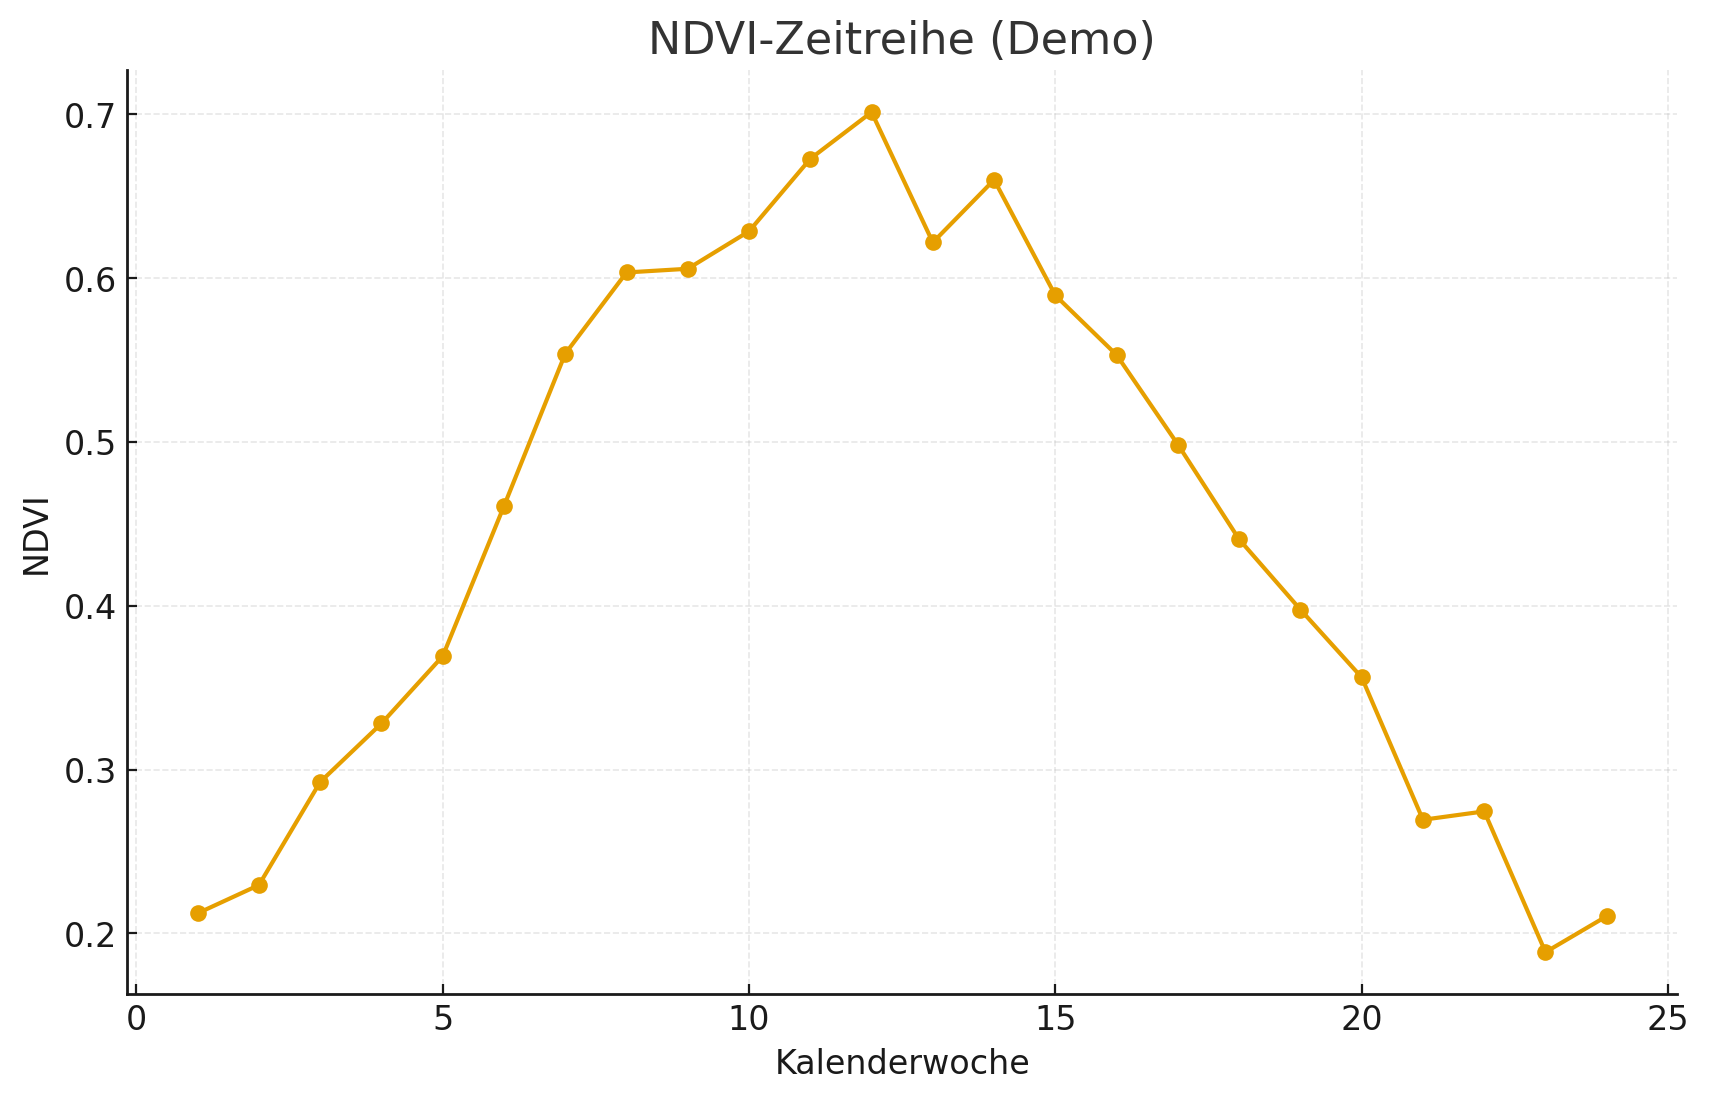
\includegraphics[width=.8\textwidth]{bilder/ndvi_demo.png}
  \caption{NDVI-Zeitreihe einer Beispielwiese. Platzhaltergrafik; bitte durch eigene Daten ersetzen.}
  \label{fig:ndvi}
\end{figure}

\section{Blatt- und Bestandsmessungen}
\subsection{Spektren am Blatt}
Reflexions- und Transmissionsmessungen zeigen die klassische „grüne Lücke“ sowie die starke Absorption im Blau und Rot. Änderungen der Pigmentgehalte verschieben die Kurven \parencite{meyer2018photosynthese}.
\begin{figure}[H]
  \centering
  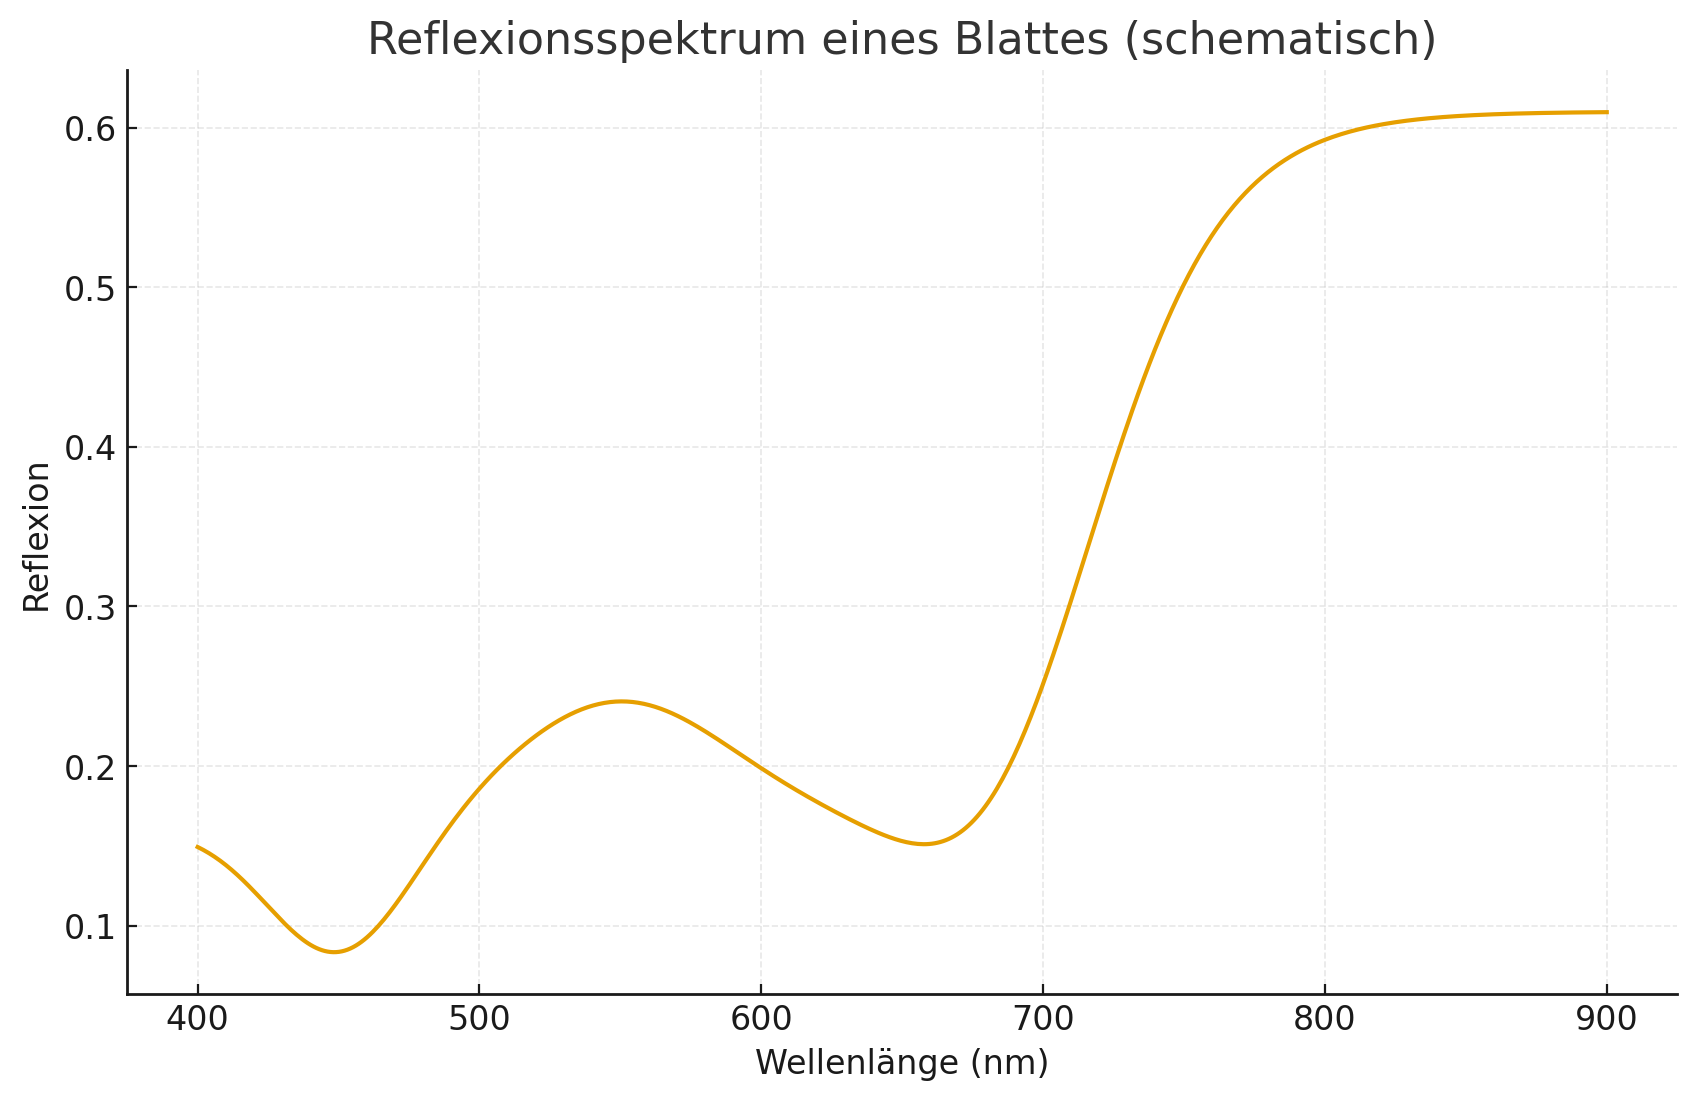
\includegraphics[width=.75\textwidth]{bilder/blattspektrum_demo.png}
  \caption{Reflexionsspektrum eines Blattes (schematisch). Platzhalter.}
  \label{fig:blatt_spektrum}
\end{figure}

\subsection{Chlorophyllfluoreszenz}
Die maximale Quantenausbeute der Photosysteme ($F_\mathrm{v}/F_\mathrm{m}$) dient als empfindlicher Stressindikator. Unter hoher Lichtlast oder Nährstoffmangel sinkt $F_\mathrm{v}/F_\mathrm{m}$ typischerweise; Photoprotektion stabilisiert das System \parencite{zhao2012chlorophyll, gao2010lightabsorption}.

\section{Fallbeispiele}
\subsection{Fall 1: Schatten vs. Sonne}
\textbf{Fragestellung}: Verändert sich die wahrgenommene Farbe und das Spektrum zwischen sonnigen und schattigen Bereichen?  
\textbf{Erwartung}: In Schattenlagen relativ höherer Grünanteil am einfallenden Licht; Blattanpassungen können zu veränderten Pigmentverhältnissen führen \parencite{zhao2012chlorophyll}.
\begin{figure}[H]
  \centering
  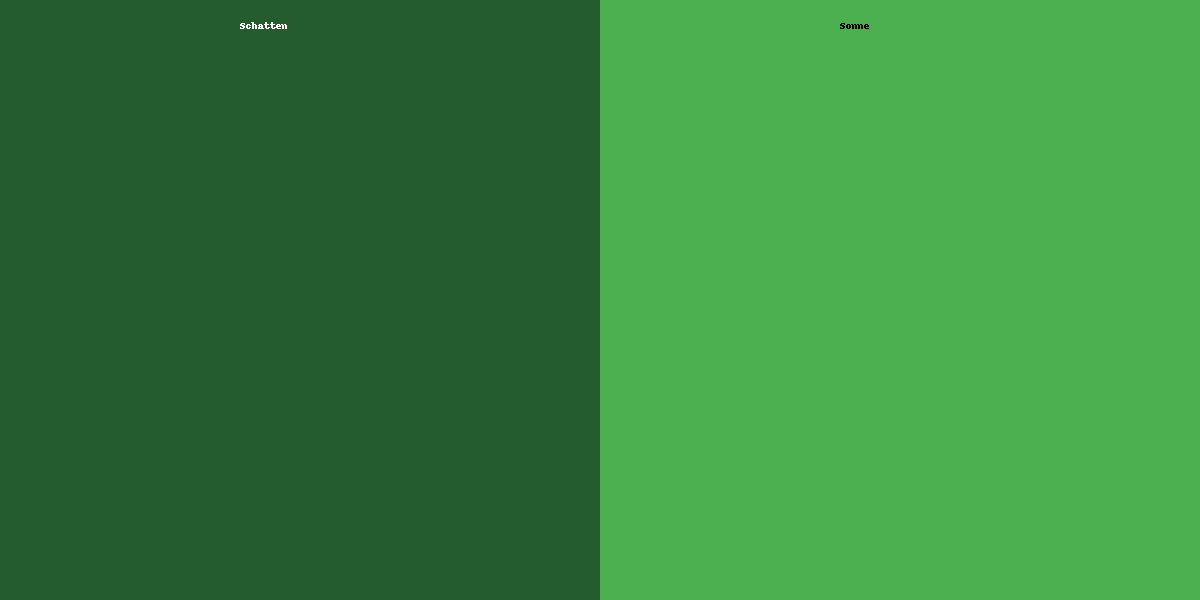
\includegraphics[width=.8\textwidth]{bilder/schatten_sonne_foto.png}
  \caption{Beispielaufnahmen: Schatten- und Sonnenbereich einer Rasenfläche. Platzhalter.}
  \label{fig:schatten_sonne}
\end{figure}

\subsection{Fall 2: Trockenstress}
\textbf{Fragestellung}: Wie reagieren Farbe und Indizes auf Wasserdefizit?  
\textbf{Erwartung}: Abnahme blattgrüner Pigmente, steigende Braun-/Gelbtöne, fallender NDVI bzw. veränderte Reflexion \parencite{gao2010lightabsorption}.
\begin{figure}[H]
  \centering
  
\includegraphics[width=.8\textwidth]{bilder/trockenstress_foto.png}
  \caption{Visuelle Veränderungen bei Trockenstress. Platzhalter.}
  \label{fig:trockenstress}
\end{figure}

\subsection{Fall 3: Düngung und Regeneration}
\textbf{Fragestellung}: Welche Veränderungen zeigen sich nach N-Düngung?  
\textbf{Erwartung}: Erhöhung des Chlorophyllgehalts, intensivere Grünfärbung, NDVI-Anstieg, ggf. höhere $F_\mathrm{v}/F_\mathrm{m}$ \parencite{schmidt2015chlorophyll}.
\begin{figure}[H]
  \centering
  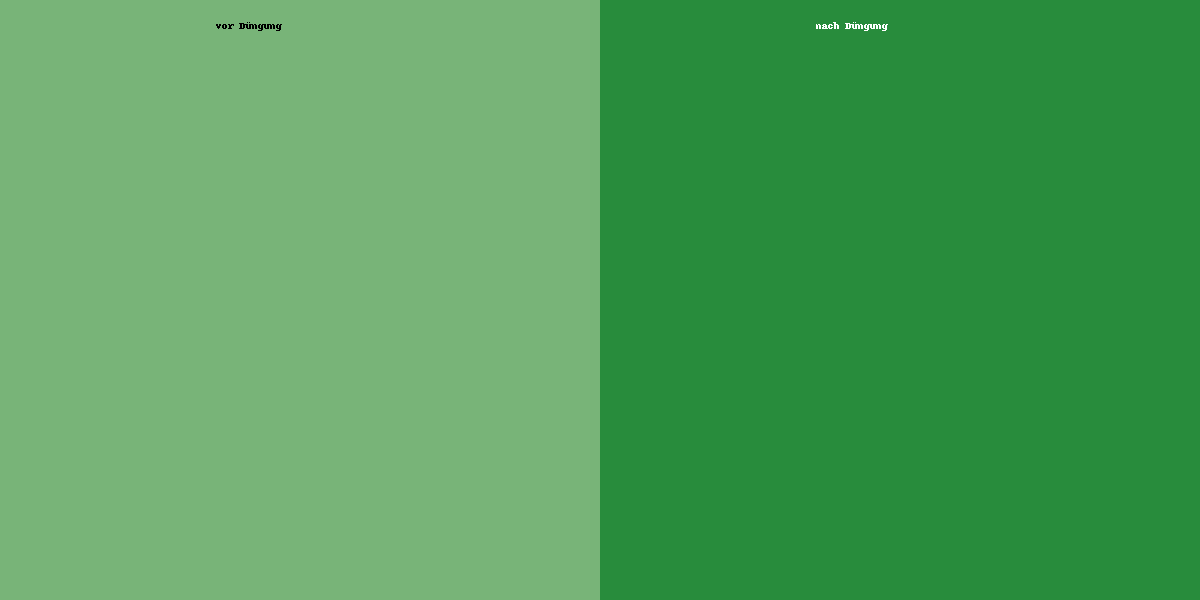
\includegraphics[width=.8\textwidth]{bilder/duengung_foto.png}
  \caption{Visuelle und spektrale Veränderungen nach Düngung. Platzhalter.}
  \label{fig:duengung}
\end{figure}

\section{Methodische Hinweise zur Reproduzierbarkeit}
\begin{itemize}
  \item \textbf{Dokumentation}: Datum, Uhrzeit, Wetter, Sonnenstand, Kameraparameter bzw. Sensorkalibration.
  \item \textbf{Referenzen}: Weißstandard/Referenztafel für Fotos; Spektronormierung für Messgeräte.
  \item \textbf{Auswertung}: Einheitliche Bildausschnitte; identische NDVI-Berechnung; Fehlerbalken für Zeitreihen.
\end{itemize}

\chapter{Diskussion}

\section{Kulturelle und kontextuelle Wahrnehmung}
Die Wahrnehmung der Farbe \textbf{Grün} ist nicht nur ein physiologischer Prozess, sondern auch kulturell und kontextuell geprägt. In vielen Gesellschaften gilt Grün als Symbol für \emph{Leben}, \emph{Frische}, \emph{Natur} und \emph{Erneuerung}. \textbf{Gras} ist dabei ein Paradebeispiel für dieses kulturelle Verständnis: Es steht sinnbildlich für \emph{Fruchtbarkeit}, \emph{Wachstum} und einen \emph{intakten Naturhaushalt}. Diese Assoziationen beeinflussen maßgeblich, wie wir die Farbe von Pflanzen, insbesondere von Gras, interpretieren \parencite{weber2016farbpsychologie}.

Während wir Gras als „natürlich grün“ empfinden, würde dieselbe Farbgebung bei anderen Organismen – etwa bei Tieren oder bestimmten Früchten – mitunter als \emph{untypisch} oder gar \emph{krankhaft} wahrgenommen werden. Das zeigt, dass unsere \textbf{Erwartungshaltung hinsichtlich Farben} stark kontextabhängig ist. Diese kulturelle Codierung ist tief im Alltag und in der Sprache verankert, was sich etwa in Redewendungen wie \emph{„alles im grünen Bereich“} oder \emph{„Grünes Licht geben“} widerspiegelt \parencite{fischer2010farbe}.

\section{Biologische Grundlage der Grünfärbung}
Auf biologischer Ebene ist die Farbgebung des Grases jedoch kein Selbstzweck, sondern eine Folge \textbf{funktionaler Optimierung}. Die grüne Farbe ergibt sich aus der selektiven Absorption von Licht durch \textit{Chlorophyll}: energiereiches \textit{rotes} und \textit{blaues Licht} wird zur Energiegewinnung genutzt, während das \textit{grüne Licht} reflektiert wird. Diese physikalische Reflexion führt zur \emph{visuellen Wahrnehmung von Grün} durch das menschliche Auge \parencite{meyer2018photosynthese}.

Neuere Studien zeigen zudem, dass Chlorophyll nicht nur der dominierende Pflanzenfarbstoff ist, sondern auch mit hoher Effizienz \textbf{Energie in Form von ATP und NADPH} umwandeln kann. Diese Moleküle sind essenziell für den anschließenden Aufbau organischer Substanzen aus anorganischem Kohlenstoff \parencite{zhao2012chlorophyll}.

\section{Evolutionäre Perspektiven und Schutzmechanismen}
Evolutionär gesehen stellt diese Anpassung einen \textbf{Überlebensvorteil} dar. Pflanzen, die ihr \textit{Lichtspektrum} effizient nutzen können, sind in der Lage, in verschiedenen Lichtverhältnissen – etwa unter direkter Sonne oder im Schatten – ausreichend Energie zu erzeugen. Es wird vermutet, dass die \textit{Dominanz von Chlorophyll-haltigen Pflanzen}, und damit auch die grüne Färbung, durch \textbf{Selektion} begünstigt wurde \parencite{schmidt2015chlorophyll}. Die vergleichsweise geringe Absorption im grünen Bereich könnte dabei auch ein \emph{Schutzmechanismus gegen Überhitzung} durch exzessive Lichtaufnahme sein \parencite{gao2010lightabsorption}.

\section{Visuelle Sensitivität und Wahrnehmungsökologie}
Zudem ist es bemerkenswert, dass die Augen vieler Tiere – darunter auch des Menschen – besonders \textbf{empfindlich für den grünen Wellenlängenbereich} sind. Diese Sensitivität liegt evolutionär vermutlich daran, dass in vegetationsreichen Umgebungen ein Großteil der Umweltinformationen im grünen Spektralbereich liegt. Ob diese Sensitivität eine \textit{Anpassung an die Umweltfarbe} oder umgekehrt ein \textbf{treibender Faktor für die grüne Ausprägung} war, ist Gegenstand wissenschaftlicher Diskussion \parencite{renoult2017evolution}.

\section{Synthese}
Insgesamt lässt sich festhalten, dass die grüne Farbe des Grases ein Resultat aus \textbf{biochemischen Prozessen}, \textbf{physikalischen Eigenschaften des Lichts} und \textbf{evolutionärer Optimierung} ist – ihre Wahrnehmung jedoch auch stark \textbf{kulturell überformt} ist. Dieses Zusammenspiel aus \emph{Naturwissenschaft} und \emph{Kultur} macht die scheinbar einfache Frage \emph{„Warum ist Gras grün?“} zu einem interdisziplinären Thema.

\chapter{Fazit}

Gras erscheint grün, weil der in Pflanzen enthaltene Farbstoff \textit{Chlorophyll} Licht in spezifischen Wellenlängen absorbiert. Insbesondere rotes und blaues Licht werden für die Photosynthese genutzt, während grünes Licht reflektiert wird. Dies ist kein zufälliger Nebeneffekt, sondern eine evolutionäre Anpassung, die Pflanzen eine möglichst effiziente Nutzung der Sonnenenergie ermöglicht. Die grüne Farbe ist somit ein sichtbares Resultat komplexer biophysikalischer Prozesse.

Darüber hinaus zeigt sich, dass die Farbwahrnehmung nicht nur biologisch erklärbar ist, sondern auch kulturell und symbolisch interpretiert wird. In vielen Gesellschaften ist die Farbe Grün tief mit Vorstellungen von Natur, Leben und Harmonie verbunden \parencite{weber2016farbpsychologie}. Diese Verknüpfung beeinflusst, wie wir natürliche Umgebungen emotional bewerten und wahrnehmen.

Trotz der umfassenden Kenntnisse über Chlorophyll gibt es weiterhin offene Fragen:

\begin{itemize}
    \item Welche Rolle spielen andere Pflanzenfarbstoffe wie \textit{Anthocyane} oder \textit{Carotinoide} bei der Farbgebung?
    \item Gibt es ökologische Vorteile für Pflanzen, die nicht grün erscheinen (z.\,B. rotblättrige Arten)?
    \item Wie wirkt sich die zunehmende Lichtverschmutzung auf die Farbwahrnehmung und Lichtnutzung von Pflanzen aus?
\end{itemize}

Diese Fragen könnten in zukünftigen Studien vertieft untersucht werden, insbesondere im Hinblick auf sich wandelnde Umweltbedingungen und genetische Anpassungsstrategien von Pflanzenarten weltweit.

\vspace{1cm}
\hrule
\vspace{0.5cm}

\noindent\textbf{Eigene Einschätzung}

\begin{quote}
Die Frage „Warum ist Gras grün?“ mag auf den ersten Blick banal erscheinen – tatsächlich verbirgt sich dahinter jedoch ein beeindruckendes Zusammenspiel aus Physik, Biologie und Kultur. Persönlich finde ich besonders faszinierend, wie ein scheinbar selbstverständliches Naturphänomen so tief in komplexe evolutionäre Mechanismen eingebettet ist. Gleichzeitig zeigt sich, dass unsere Wahrnehmung stark kulturell geprägt ist. Dass wir „grün“ mit „gut“ oder „lebendig“ assoziieren, ist nicht biologisch notwendig, sondern ein soziales Konstrukt – und das macht den Blick auf eine Wiese beim Sonnenuntergang nicht weniger schön, sondern vielleicht sogar bewusster.
\end{quote}

\vspace{0.5cm}
\hrule



\listoffigures

\printbibliography


\end{document}
